\chapter{Organization of Iconc}

The Icon compiler, iconc, takes as input the source code for an Icon
program and, with the help of a C compiler and linker, produces an
executable file. The source code may be contained in several files,
but iconc does not support separate compilation. It processes an
entire program at once. This requirement simplifies several of the
analyses, while allowing them to compute more accurate
information. Without the entire program being available, the effects
of procedures in other files is unknown. In fact, it is not possible
to distinguish built-in functions from missing procedures. Type
inferencing would be particularly weakened. It would have to assume
that any call to an undeclared variable could have any side effect on
global variables (including procedure variables) and on any data
structure reachable through global variables or parameters.


\section[18.1 Compiler Phases]{18.1 Compiler Phases}

Iconc is organized into a number of phases. These are illustrated in
the diagram on the following page.

The initialization phase includes reading a data base of information
about run-time routines into internal tables. This information is used
in many of the other phases.

The source analysis phase consists of a lexical analyzer and
parser. These are adapted from those used in the interpreter
system. The parser generates abstract syntax trees and symbol tables
for all procedures before subsequent phases are invoked. The symbol
resolution phase determines the scope of variables that are not
declared in the procedures where they are used. This resolution can
only be done completely after all source files for the program are
read. If a variable does not have a local declaration, the compiler
checks to see whether the variable is declared global (possibly as a
procedure or record constructor) in one of the source files. If not,
the compiler checks to see whether the variable name matches that of a
built-in function. If the name is still not resolved, it is considered
to be a local variable.

%--% 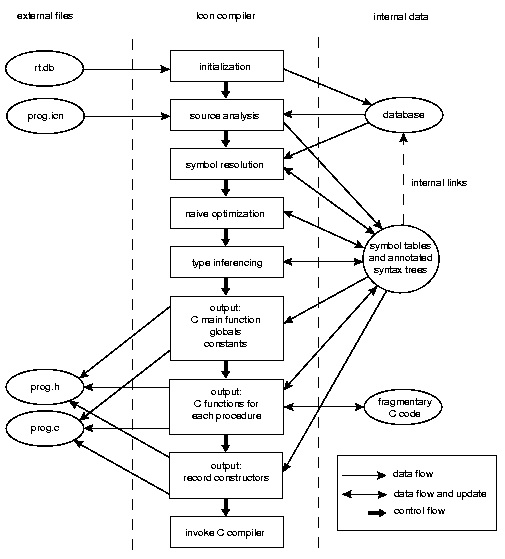
\includegraphics[width=5.5484in,height=5.822in]{kw/figure6-1.png}  

\noindent
\begin{figure}
\begin{tikzpicture}[draw,very thick,font=\small\tt,>=Latex,arrows=->,
    box/.style={rectangle, minimum width=4cm, thick, minimum height=0.9cm,draw},
    elps/.style={ellipse,ellipse,draw,minimum width=2cm},
]`
%  \draw[help lines] (0,0) grid (15,15);

% column headers
  \node at (1,15) {external files};
  \node at (7,15) {Icon compiler};
  \node at (13.5,15) {internal data};
  \foreach \x in {3.75, 10.25} {
    \draw[-,dashed, dash pattern=on 0.3cm off 0.3cm, line width=1.4pt]
        (\x,15) -- (\x, -0.5);
  };
  
% draw the boxes and ellipses
  \node(rtdb)[elps] at (1,14)      {rt.db};
  \node(progicn)[elps] at (1,12.5)   {prog.icn};
  \node(database)[elps] at (13.5,12.5) {database};
  \node(symt) at (13.5,8) [elps, align=center]
       {symbol tables\\and annotated\\syntax trees};
  \node(init)[box] at (7,14)   {initialization};
  \node(src)[box] at (7,12.5)  {source analysis};
  \node(symres)[box] at (7,11) {symbol resolution};
  \node(naio)[box] at (7,9.5)  {naive optimization};
  \node(ti)[box] at (7,8)      {type inferencing};
  \node(opm)[box,align=center] at (7,6)
       {output{:}\\C main function\\globals\\constants};
  \node(opf)[box,align=center] at (7,3.5)
       {output{:}\\C functions for\\each procedure};
  \node(progh)[elps] at (1,4)  {prog.h};
  \node(progc)[elps] at (1,3)  {prog.c};
  \node(frags)[elps, align=center] at (13.5,3.5) {fragmentary\\C code};
  \node(opr)[box,align=center] at (7,1.5)
       {output{:}\\record constructors};
  \node(cc)[box] at (7,0)    {invoke C compiler};

% Connect compiler boxes to files etc.
  \draw (rtdb) -- (init); \draw (init.east) -- (database);
  \draw (progicn) -- (src);
  \draw (database) -- (src); \draw (database) -- (node cs:name=symres,angle=5);
  \draw (node cs:name=src,angle=-5) -- (symt);
  \draw [<->] (node cs:name=symres,angle=-5) -- (symt);
  \draw [<->] (naio.east) -- (symt);
  \draw [<->] (ti.east) -- (symt);
  \draw[loosely dashed] (symt) -- node[right=0.3,align=center]
       {internal\\links} (database);
  \draw (symt) -- (opm.east);
  \draw [<->] (symt) -- (node cs:name=opf, angle=10);
  \draw (symt) -- (opr.east);
  \draw (node cs:name=opm, angle=160) -- (node cs:name=progh, angle=20);
  \draw (node cs:name=opm, angle=200) -- (node cs:name=progc, angle=10);
  \draw (node cs:name=opf, angle=166) -- (progh);
  \draw (node cs:name=opf,angle=194) --  (progc);
  \draw (node cs:name=opr, angle=170) -- (node cs:name=progh, angle=340);
  \draw (node cs:name=opr, angle=190) -- (node cs:name=progc, angle=350);
  \draw [<->] (opf) -- (frags);

% Draw the flow of control
  \begin{scope}[line width=1.8pt, >=Stealth]
    \draw (init) -- (src);
    \draw (src) -- (symres);
    \draw (symres) -- (naio);
    \draw (naio) -- (ti);
    \draw (ti) -- (opm);
    \draw (opm) -- (opf);
    \draw (opf) -- (opr);
    \draw (opr) -- (cc);
% whilst the foc arrows are set up, draw the foc key arrow
    \draw (11.45,0.5) -- (12.2,0.5);
  \end{scope}


% draw the key block
  \draw (11.1,1.6) -- (12.2,1.6);
 \node[anchor=west] at (12.25,1.6) {data flow};
  \draw[<->] (11.1,1) -- (12.2,1);
  \node[anchor=west] at (12.25,1) {data flow and update};
   \node[anchor=west] at (12.25,0.5) {control flow};
  \draw[thin] (11,0) rectangle (16.2,2);
  
\end{tikzpicture}
\caption{Compiler phases and data flow}
\end{figure}

\section[18.2 Naive Optimizations]{18.2 Naive Optimizations}

Naive optimizations involve invocation and assignment. These
optimizations are done before type inferencing to aid that
analysis. Certain ``debugging features'' of Icon such as the
variable function interfere with these optimizations. By default,
these features are disabled. If the user of iconc requests the
debugging features, these optimizations are bypassed. While these
optimizations are being done, information is gathered about whether
procedures suspend, return, or fail. This information is used in
several places in the compiler.

The invocation optimization replaces general invocation by a direct
form of invocation to a procedure, a built-in function, or a record
constructor. This optimization involves modifying nodes in the syntax
tree. It only applies to invocations where the expression being
invoked is a global variable initialized to a value in one of the
three classes of procedure values. First, the Icon program is analyzed
to determine which variables of this type appear only as the immediate
operands of invocations. No such variable is ever assigned to, so it
retains its initial value throughout the program (a more exact
analysis could be done to determine the variables that are not
assigned to, but this would seldom yield better results in real Icon
programs because these programs seldom do anything with procedure
values other that invoke them). This means that all invocations of
these variables can be replaced by direct invocations. In addition,
the variables themselves can be discarded as they are no longer
referenced.

The invocation optimization improves the speed of type inferencing in
two ways, although it does nothing to improve the accuracy of the
information produced. Performing type inferencing on direct
invocations is faster than performing it on general invocations. In
addition, type inferencing has fewer variables to handle, which also
speeds it up.

The invocation optimization does improve code generated by the
compiler. In theory, the optimization could be done better after type
inferencing using the information from that analysis, but in practice
this would seldom produce better results. On most real Icon programs,
this optimization using the naive analysis replaces all general
invocations with direct ones.

As noted in Chapter 15, it is important for type inferencing to
distinguish strong updates from weak updates. The data base contains a
general description of assignment, but it would be difficult for a
type inferencing system to use the description in recognizing that a
simple assignment or an augmented assignment to a named variable is a
strong update.  It is much easier to change general assignments where
the left hand side is a named variable to a special assignment and
have type inferencing know that the special assignment is a strong
update. Special-casing assignment to named variables is also important
for code generation. General optimizations to run-time routines are
not adequate to produce the desired code for these assignments. The
optimizations to assignment are described in Chapter 22.

The details of type inferencing are described in other
chapters. Producing code for the C main function, global variables,
constants, and record constructors is straightforward. C code is
written to two files for organizational purposes; it allows
definitions and code to be written in parallel.


\section[18.3 Code Generation for Procedures]{18.3 Code Generation for Procedures}

Producing code for procedures involves several sub-phases. The
sub-phases are liveness analysis, basic code generation, fix-up and
peephole optimization, and output. During this phase of code
generation, procedures are processed one at at time.

These sub-phases are described in later chapters. The code fix-up
phase and peephole optimization are performed during the same pass
over the internal representation of the C code. Some clean-up from
peephole optimization is performed when the code is written. The
logical organization of the compiler places the fix-up phase as a pass
in code generation with peephole optimization being a separate
phase. The organization of this dissertation reflects the logical
organization of the compiler rather than its physical organization.

The physical organization of this phase is shown in the following diagram.

%--%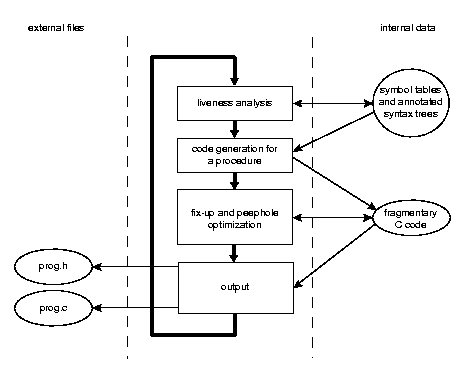
\includegraphics[width=5.1311in,height=3.9063in]{kw/figure6-2.png} 

\noindent
\begin{figure}[hb]
\begin{tikzpicture}[draw,very thick,font=\small\tt,>=Latex,arrows=->,
    box/.style={rectangle, minimum width=4cm, thick, minimum height=1.4cm,draw},
    elps/.style={ellipse,ellipse,draw,minimum width=2cm},
]`
%  \draw[help lines] (0,2) grid (15,13);

% column headers
  \node at (1,13) {external files};
  \node at (13.5,13) {internal data};
  \foreach \x in {3.5, 10.5} {
    \draw[-,dashed, dash pattern=on 0.3cm off 0.3cm, line width=1.4pt]
        (\x,13) -- (\x, 2);
  };
  
% draw the boxes and ellipses
  \node(symt) at (13.5,11) [elps, align=center]
       {symbol tables\\and annotated\\syntax trees};
  \node(la)[box] at (7,11)  {liveness analysis};
  \node(cg)[box,align=center] at (7,8.5)      {code generation for\\a procedure};
  \node(fix)[box,align=center] at (7,6)
       {\\fix-up and peephole\\optimization\\};
  \node(op)[box,align=center] at (7,3.5)
       {\\output\\};
  \node(progh)[elps] at (1,4)  {prog.h};
  \node(progc)[elps] at (1,3)  {prog.c};
  \node(frags)[elps, align=center] at (13.5,6) {fragmentary\\C code};

% Connect compiler boxes to files etc.
  \draw[<->] (la) -- (symt);
  \draw (symt) -- (node cs:name=cg, angle=10);
  \draw (node cs:name=cg,angle=350) -- (frags);
  \draw [<->] (frags) -- (fix);
  \draw (frags) -- (op.east);
  \draw (node cs:name=op,angle=166) -- (progh);
  \draw (node cs:name=op, angle=194) -- (progc);

% Draw the flow of control
  \begin{scope}[line width=2.5pt, >=Stealth]
    \draw (la) -- (cg);
    \draw (cg) -- (fix);
    \draw (fix) -- (op);
    \draw (op) -- (7,2) -- (4.2,2) -- (4.2,12.5) -- (7,12.5) -- (la);
  \end{scope}

\end{tikzpicture}
\caption{The physical organization of the code generation phase}
\end{figure}

\bigskip


\bigskip

